% This is a comment!

% This is the document declaration (with default fontsize)
\documentclass[12pt]{article}

% these are some useful packages. these add functionality to your document
\usepackage{amssymb}
\usepackage{amsthm}
\usepackage{amssymb}
\usepackage{amsmath}  % math symbols
\usepackage{mathdots}
\usepackage[pdftex]{graphicx}
\usepackage{fancyhdr}
%\usepackage[margin=1in]{geometry}
\usepackage{multicol}
\usepackage{bm}
\usepackage{listings}
\PassOptionsToPackage{usenames,dvipsnames}{color}  %% Allow color names
\usepackage{pdfpages}
\usepackage{algpseudocode}
\usepackage{tikz}
\usetikzlibrary{automata,positioning}
\usepackage{enumitem}
\usepackage[T1]{fontenc}
\usepackage{inconsolata}
\usepackage{framed}
\usepackage{wasysym}
\usepackage[thinlines]{easytable}
\usepackage{wrapfig}  % in case you want to use a figure
\usepackage{hyperref} % add hyper links
\usepackage{minted}

% This package controls the margins of the page.
\usepackage[top=1in, bottom=1in, left=0.8in, right=1in]{geometry}

\usepackage{multicol} % in case you want to use multiple columns
\setlength{\columnsep}{0.1pc}

% document headers!
\title{CS 109: Introduction to Probability for Computer Scientists\\Problem Set \#6}
\author{\Large{author}} % Replace with your own name!!!
\date{\Large{\today}} % today does the right thing

\lhead{author} % Replace with your own name!!!
\chead{Problem Set \#6}
\rhead{\today}

\newcommand{\abs}[1]{\lvert #1 \rvert}
\newcommand{\absfit}[1]{\left\lvert #1 \right\rvert}
\newcommand{\norm}[1]{\left\lVert #1 \right\rVert}
\newcommand{\eval}[3]{\left[#1\right]_{#2}^{#3}}
\renewcommand{\(}{\left(}
\renewcommand{\)}{\right)}
\newcommand{\floor}[1]{\left\lfloor#1\right\rfloor}
\newcommand{\ceil}[1]{\left\lceil#1\right\rceil}
\newcommand{\pd}[1]{\frac{\partial}{\partial #1}}
\newcommand{\inner}[1]{\langle#1\rangle}
\newcommand{\cond}{\bigg|}
\newcommand{\rank}[1]{\mathbf{rank}(#1)}
\newcommand{\range}[1]{\mathbf{range}(#1)}
\newcommand{\nullsp}[1]{\mathbf{null}(#1)}
\newcommand{\repr}[1]{\left\langle#1\right\rangle}

\DeclareMathOperator{\Var}{Var}
\DeclareMathOperator{\tr}{tr}
\DeclareMathOperator{\Tr}{\mathbf{Tr}}
\DeclareMathOperator{\diag}{\mathbf{diag}}
\DeclareMathOperator{\dist}{\mathbf{dist}}
\DeclareMathOperator{\prob}{\mathbf{prob}}
\DeclareMathOperator{\dom}{\mathbf{dom}}
\DeclareMathOperator{\E}{\mathbf{E}}
\DeclareMathOperator{\R}{\mathbb{R}}
\DeclareMathOperator{\var}{\mathbf{var}}
\DeclareMathOperator{\quartile}{\mathbf{quartile}}
\DeclareMathOperator{\conv}{\mathbf{conv}}
\DeclareMathOperator{\VC}{VC}
\DeclareMathOperator*{\argmax}{arg\,max}
\DeclareMathOperator*{\argmin}{arg\,min}
\DeclareMathOperator{\Ber}{Bernoulli}
\DeclareMathOperator{\NP}{\mathbf{NP}}
\DeclareMathOperator{\coNP}{\mathbf{coNP}}
\DeclareMathOperator{\TIME}{\mathsf{TIME}}
\DeclareMathOperator{\polytime}{\mathbf{P}}
\DeclareMathOperator{\PH}{\mathbf{PH}}
\DeclareMathOperator{\SIZE}{\mathbf{SIZE}}
\DeclareMathOperator{\ATIME}{\mathbf{ATIME}}
\DeclareMathOperator{\SPACE}{\mathbf{SPACE}}
\DeclareMathOperator{\ASPACE}{\mathbf{ASPACE}}
\DeclareMathOperator{\NSPACE}{\mathbf{NSPACE}}
\DeclareMathOperator{\Z}{\mathbb{Z}}
\DeclareMathOperator{\N}{\mathbb{N}}
\DeclareMathOperator{\EXP}{\mathbf{EXP}}
\DeclareMathOperator{\NEXP}{\mathbf{NEXP}}
\DeclareMathOperator{\NTIME}{\mathbf{NTIME}}
\DeclareMathOperator{\DTIME}{\mathbf{DTIME}}
\DeclareMathOperator{\poly}{poly}
\DeclareMathOperator{\BPP}{\mathbf{BPP}}
\DeclareMathOperator{\ZPP}{\mathbf{ZPP}}
\DeclareMathOperator{\RP}{\mathbf{RP}}
\DeclareMathOperator{\coRP}{\mathbf{coRP}}
\DeclareMathOperator{\BPL}{\mathbf{BPL}}
\DeclareMathOperator{\IP}{\mathbf{IP}}
\DeclareMathOperator{\PSPACE}{\mathbf{PSPACE}}
\DeclareMathOperator{\NPSPACE}{\mathbf{NPSPACE}}
\DeclareMathOperator{\SAT}{\mathsf{SAT}}
\DeclareMathOperator{\NL}{\mathbf{NL}}
\DeclareMathOperator{\PCP}{\mathbf{PCP}}
\DeclareMathOperator{\PP}{\mathbf{PP}}
\DeclareMathOperator{\cost}{cost}
\let\Pr\relax
\DeclareMathOperator*{\Pr}{\mathbf{Pr}}

\theoremstyle{definition}
\newtheorem*{answer}{Answer}

\definecolor{shadecolor}{gray}{0.95}

\setlength{\parindent}{0pt}

\pagestyle{fancy}

\renewcommand{\thefootnote}{\fnsymbol{footnote}}

% begin the document
\begin{document}

% actually insert the title.
\maketitle

\begin{enumerate}
\large{
    %1
    \item Consider a sample of I.I.D. random variables $X^{(1)}$, $X^{(2)}$, $\ldots$, $X^{(n)}$, where each $X^{(i)} \sim \text{Exp}(\lambda)$. Derive the maximum likelihood estimate for the parameter $\lambda$ in the Exponential distribution.
    
    \begin{shaded}
    \begin{answer}
    
    \end{answer}
    \end{shaded}
    \newpage
    
    %2
    \item Say you have a set of binary input features/variables X$_1$, X$_2$, $\ldots$, X$_m$ that can be used to make a prediction about a discrete binary output variable Y (i.e., each of the X$_i$ as well as Y can only take on the values 0 or 1). Say that the first $k$ input variables X$_1$, X$_2$, $\ldots$, X$_k$ are actually all \textit{identical} copies of each other, so that when one has the value 0 or 1, they all do. Explain informally, but precisely, why this may be problematic for the model learned by the Naive Bayesian Classifier.
    
    \begin{shaded}
    \begin{answer}
    
    \end{answer}
    \end{shaded}
    \newpage
    
    %3
    \item \textit{Note: Because of Spring quarter, you won't be able to answer this question until May 31st. You can (and should) skip it, do the programming problems, and come back to it later.}\\ \\
    Consider this four neuron neural-network that is trained on $n$ data points ($x^{(i)}, y^{(i)}$):\\ \\
    
    \begin{center}
    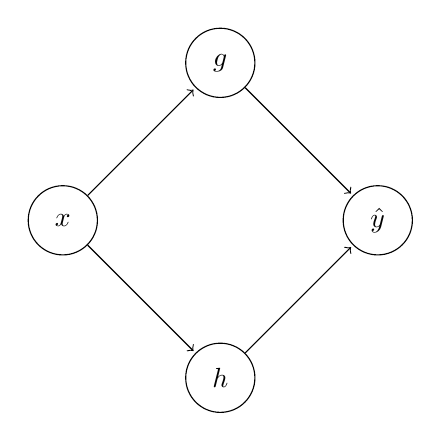
\begin{tikzpicture}[shorten >=1pt,node distance=2cm,on grid,auto] 
    % \node[state, options?] (identifier) [placement] {display};
    \node[] (0) [] {};
    \node[state] (1) [below=of 0] {$x$};
    \node[state] (2) [right=of 0] {$g$};
    \node[] (3) [below=of 2] {};
    \node[state] (4) [below=of 3] {$h$}; 
    \node[state] (5) [right=of 3] {$\hat{y}$}; 
                      
    % (start identifier) edge [options?] node {display label} (target identifier)
    % 		                edge [options?] node {display label} (another target identifier)
    \path[->]
    (1) edge node {} (2)
        edge node {} (4)
    (2) edge node {} (5)
    (4) edge node {} (5);
    \end{tikzpicture}
    
    $g$ = sigmoid($\theta_1 \cdot x$)\\
    $h$ = sigmoid($\theta_2 \cdot x$)\\
    $\hat{y}$ = sigmoid($\theta_3 \cdot g + \theta_4 \cdot h$)\\
    $LL(\theta) = \displaystyle \sum_{i=1}^n y^{(i)}\ \text{log}\ \hat{y}^{(i)} + (1 - y^{(i)})\ \text{log} (1 - \hat{y}^{(i)})$
    \end{center}
    
    \begin{enumerate}
        \item Calculate the gradients of the log-likelihood function with respect to all four parameters.
        \item Explain in a few sentences how you could use the function that you calculated in part (a) to train the neural network. 
    \end{enumerate}
    
    \begin{shaded}
    \begin{answer}
    
    \end{answer}
    \end{shaded}
    \newpage
    
    %4
    \textbf{Programming Problems}\\ \\
    \small{
    For the following problems, you will be implementing two learning algorithms: the Naive Bayesian Classifier and Logistic Regression. You may implement your algorithms any language, though we will only be offering programming help for python. You can feel free (but are under no obligation) to use standard libraries. You should \textbf{not} use any library that actually implements machine learning algorithms. For each algorithm, \textbf{you should turn in your source code as well as answers to the questions listed below}. It's fine if your implementation of both algorithms is in a single file or if you use multiple files. In either case, please provide any code you write.\\
    
    For each algorithm you write, you will be testing it with three data sets. A description of the data sets you will be using, the file format for the data files, and instructions on how to obtain the data files are given below. Note: you do \textbf{not} need to do any error checking in your file reading code (you can assume the data is always correctly formatted). To simplify your implementation, you can assume that all input features are always binary variables (0 or 1), and the output class is also always a binary variable (0 or 1). For the assignment, our main interest is that you understand how the machine learning algorithms work. As a result, you do not need to worry about the generality of your implementation --- i.e., you can write your algorithms to only deal with binary input/output features. Your code should, however, be general enough to work for any number of input features or data instances (within reason), as the different datasets you will be dealing with contain different numbers of input features and data instances. We will be grading your code only on functionality, not on programming style. With that said, it is still in your interest to write good modular code as there are many opportunities for code reuse in implementing this assignment.\\
    
    \textbf{Training and testing your algorithms}\\
    The ``training'' data files should be used to train your learning algorithm (i.e., determine the model parameters). The ``testing'' data file should be used to determine the accuracy of your model \textit{after} the training phase is complete. In other words, when we describe \textit{training} an algorithm below, you should take that to mean that you are working \textit{only} with the ``\texttt{-train}'' file for a particular dataset to determine the parameters of your model. When we then describe \textit{testing} a model you should take that to mean that you are using only the ``\texttt{-test}'' file for a particular dataset to determine how well your model does at classifying the data.\\
    
    \textbf{Measuring model accuracy}\\
    After a model is trained, we determine its accuracy by testing it on a new set of data (generally not the same data we used to train the model). We measure the model's accuracy by determining how many of the testing vectors were correctly classified --- that is, the number of times the output class value predicted by the model was the same as the actual output class value provided in the data. We report accuracy by indicating the number of data vectors that were tested of each class, and the number that were correctly classified. For example, say we have a testing data set consisting of 12 vectors total, where the first 5 vectors are of class $y$ = 0 and the remaining 7 of class $y$ = 1. When we then make predictions for each data vector using our model, say we correctly predict class $\hat{y}$ = 0 for 4 out of the first 5 vectors and then correctly predict class $\hat{y}$ = 1 for 5 out of the next 7 vectors. Our overall accuracy for the model would be 0.75 since we correctly classified a total of 9 out of 12 vectors. We would report these results as follows:\\
    \texttt{Class 0: tested 5, correctly classified 4\\
    Class 1: tested 7, correctly classified 5\\
    Overall: tested 12, correctly classified 9\\
    Accuracy = 0.75}\\
    You should use this same accuracy reporting scheme for the algorithms you implement below.}
    
    \large{
    \newpage
    \item Implement the Naive Bayesian Classifier for binary input/output data. Specifically, your classifier should make predictions for the output variable using the rule: $\hat{Y} = \text{argmax}_y P(\textbf{X}\ |\ Y)P(Y)$, by employing the Naive Bayes assumption, which states that:
    \[
    P(\textbf{X}|Y) = P(X_1, X_2, \ldots, X_m|Y) = \prod_{i=1}^m P(X_i|Y)
    \]
    Thus, your program will need to estimate the values P(Y) as well as P(X$_i$ | Y) for all $1 \leq i \leq m$ from the training data. Note that to estimate the probability mass function P(X$_i$ | Y), you will need to estimate both P(X$_i$ | Y = 0) and P(X$_i$ | Y = 1).
    
    \begin{enumerate}
        \item Train your algorithm on the data file \texttt{simple-train.txt}. Test your algorithm on the data file \texttt{simple-test.txt} and report your classification accuracy. Run your algorithm once with Maximum Likelihood Estimators (MLE) and once with Laplace Estimators. As a sanity check, you should be able to achieve 100\% classification accuracy on the testing data using a model trained with Maximum Likelihood Estimators.
        \item Train your algorithm on the data file \texttt{netflix-train.txt}. Test your algorithm on the data file \texttt{netflix-test.txt}. Run your algorithm twice, once with MLE and once with Laplace Estimators. For both versions of Naive Bayes, answer the following questions:
        \begin{enumerate}
            \item What is your estimate for P(Y = 1)?
            \item For all values of $i$, what is your estimate P(X$_i$ = 1 | Y = 1)?
            \item For all values of $i$, what is your estimate P(X$_i$ = 1 | Y = 0)?
            \item Report your classification accuracy for both MLE and Laplace estimators.
        \end{enumerate}
        \item For Naive Bayes trained on netflix-train.txt with an MLE estimator answer the following questions:
        \begin{enumerate}
            \item Using the probabilities that you estimated for Naive Bayes, decide which five movies are the most indicative that a user will like Love Actually. In other words, for which five movies is the ratio P(Y = 1 | X$_i$ = 1) / P(Y = 1 | X$_i$ = 0) the largest.
            \item Give one example of a miss-prediction. Try and explain what went wrong.
        \end{enumerate}
        \item Train your algorithm on the data file \texttt{ancestry-train.txt}. Test your algorithm on the data file \texttt{ancestry-test.txt} and report your classification accuracy. Again, remember to do this once with Maximum Likelihood Estimators and once with Laplace Estimators.
        \item Train your algorithm on the data file \texttt{heart-train.txt}. Test your algorithm on the data file \texttt{heart-test.txt} and report your classification accuracy. Again, remember to do this once with Maximum Likelihood Estimators and once with Laplace Estimators.
        \item Include a copy of your code for the Naive Bayes Classifier.
    \end{enumerate}
    
    \begin{shaded}
    \begin{answer}
    
    \end{answer}
    \end{shaded}
    
    \newpage
    
    %5
    \item Implement Logistic Regression for binary input/output data. Specifically, you should implement the gradient ascent algorithm described in class.\\ \\
    Note that you will need to use an exponential function ($e^x$) to implement Logistic Regression. In Python, you will find the function \texttt{exp(x)} from the library \texttt{math} helpful.
    
    \begin{enumerate}
        \item Train your algorithm on the data file \texttt{simple-train.txt}. Use learning rate $\eta$ = 0.0001 and 10,000 training steps. Test your algorithm on the data file \texttt{simple-test.txt} and report your classification accuracy. You should be able to achieve 100\% classification accuracy on the testing data.
        \item Train your algorithm on the data file \texttt{netflix-train.txt}. Use learning rate $\eta$ = 0.0001 and 3,000 training steps. Test your algorithm on the data file \texttt{netflix-test.txt}:
        \begin{enumerate}
            \item Report your final parameter weights after training.
            \item Report your classification accuracy.
            \item According to the weights of your logistic regression function, which five movies are the strongest predictors that a user will like Love Actually?
            \item What is the log likelihood of the training data when all the parameters are 0?
            \item What is the log likelihood of the training data after training?
        \end{enumerate}
        
        \item Train your algorithm on the data file \texttt{ancestry-train.txt}. Use learning rate $\eta$ = 0.0001 and 10,000 training steps. Test your algorithm on the data file \texttt{ancestry-test.txt} and report your classification accuracy.
        \item Train your algorithm on the data file \texttt{heart-train.txt}. Experiment with using different learning rates $\eta$, where you are still testing your algorithm on the data file \texttt{heart-test.txt}. Each time use 10,000 training steps. As a starting point for experimenting, try $\eta$ = 0.0005 and $\eta$ = 0.00002 (i.e., values for $\eta$ that are larger and smaller than 0.0001 by a factor of 5), and then continue experimenting from there. Report the highest classification accuracy you could obtain on the testing data, and what was the value of the learning rate $\eta$ you used to obtain it. Explain why do you think the learning rate had such an effect on your classification accuracy.
        \item Include a copy of your code for Logistic Regression.
    \end{enumerate}
    
    \begin{shaded}
    \begin{answer}
    
    \end{answer}
    \end{shaded}
    \newpage
    
    %6
    \item \text{[Extra credit]} For extra credit, try to write a simple neural network algorithm (or even train a Bayesian Network). Train on the data file \texttt{netflix-train.txt}. Report the maximum accuracy that you were able to obtain for the data file \texttt{netflix-test.txt}.
    
    \begin{shaded}
    \begin{answer}
    
    \end{answer}
    \end{shaded}
    
}}
\end{enumerate}


\end{document}